\documentclass{article}
\documentclass{bar}
\usepackage{graphicx}
\usepackage[utf8]{inputenc}
\usepackage[fleqn]{amsmath}
\usepackage{titling}
\usepackage{graphicx,wrapfig,lipsum}
\usepackage{amssymb}
\usepackage{listings}
\usepackage{mathtools}
\usepackage[font=small,labelsep=none]{caption}
\usepackage{hyperref}

\setlength{\droptitle}{-10em}
\setlength\parindent{0pt}

\title{Project 1 - FYS3150}\vspace{-3ex}
\author{Emil Helland Broll, Benedicte Allum Pedersen,\\ Fredrik Oftedal Forr}
\date{\vspace{-5ex}}

\begin{document}
\maketitle

\subsection*{Introduction}
In this report we will address several ways of solving linear equations. The different algorithms that will be used are Thomas algorithm and LU decomposition. The Thomas algorithm is found from a general expression and the way it was done is represented further down in this report. To perform the LU decomposition the package armadillo for c++ was used. The links for the codes we have made are found in the appendix.

\vspace{0.3cm}

The equation wich we have solved is the Poisson's equation wich is a classical equation from electromagnetism, in three dimensions the equation is:
\begin{equation*}
\nabla^2 \Phi = -4\pi \rho (\mathbf{r}).
\end{equation*}

where $\Phi$ is the electrostatic potential generated by a localized charge distribution $\rho (\mathbf{r})$. If $\Phi$ and $\rho (\mathbf{r})$ are spherical symmetrical, and we do the substitution $\Phi(r)= \phi(r)/r$, the equation simplifies to:
\begin{equation*}
\frac{d^2\phi}{dr^2}= -4\pi r\rho(\mathbf{r}).
\end{equation*}

If we let $f = -4\pi r \rho (\mathbf{r})$, and by let $\phi\rightarrow u$ and
$r\rightarrow x$, the general one-dimensional Poisson equation will read:
\begin{equation*}
-u''(x) = f(x).
\end{equation*}

\subsection*{Project 1 a)}

\noindent We have solved the one-dimensional Poisson equation with Dirichlet boundary conditions and by rewriting it as a set of linear equations.

\noindent We let the discretized approximation to $u$ be defined as $v_i$. The second derivative of $u$ is then defined as:
\[
&-\frac{v_{i+1}+v_{i-1}-2v_i}{h^2} = f_i
\]
where $h$ is the step length and is defined as $h=1/(n+1)$ and where $f_i = f(x_i)$.
We can rewrite this equation to a set of linear equations like this:
\begin{flalign*}
   &-\frac{v_{i+1}+v_{i-1}-2v_i}{h^2} = f_i\\
   &-(v_{i+1}+v_{i-1}-2v_i) = f_ih^2\\
   &2v_i -v_{i+1}-v_{i-1}=f_ih^2
\end{flalign*}
Wich expands to
\begin{flalign*}
  2v_1 - v_0 - v_2 &= f_1h^2\\
  2v_2 - v_1 - v_2 &= f_2h^2\\
  &\vdots\\
  2v_n - v_{n-1} - v_n+1 &= f_3h^2\\
\end{flalign*}
The boundary conditions give us $v_{n+1}=u(1)=0$ and $v_0=u(0)=0$. We also introduce $f_ih^2 = g_i$. We can then write this expression as
\begin{flalign*}
  \begin{bmatrix}
    2 & -1 & 0 &\dots & 0 & 0\\
    -1 & 2 & -1 & \dots & 0 & 0\\
    0 & -1 & 2 & \dots & 0 & 0 \\
    \vdots & \vdots & \vdots & \ddots & \vdots & \vdots \\
    0 & 0 & 0 &\dots& 2 & -1\\
    0 & 0 & 0 &\dots& -1 & 2
  \end{bmatrix}
  \begin{bmatrix}
    v_1\\
    v_2\\
    v_3\\
    \vdots\\
    v_{n-1}\\
    v_n
  \end{bmatrix} =
  \begin{bmatrix}
    g_1\\
    g_2\\
    g_3\\
    \vdots\\
    g_{n-1}\\
    g_n
  \end{bmatrix}
\end{flalign*}


\subsection*{Project 1 b)}
We rewrite our matrix A in terms of one-dimensional vectors $a$ and $c$ of length 1 : $n-1$ and $a$ of length 1 : $n$;
\begin{flalign*}
  \mathbf{A}=\begin{bmatrix}
    b_1 & c_1 & 0 &\dots & \dots & 0 \\
    a_1 & b_2 & c_2 & \dots & \dots & 0 \\
    0 & a_2 & b_3 & c_3 & \dots \dots & 0  \\
    \vdots & \vdots & \vdots & \ddots & \vdots & \vdots \\
    0 & 0 &\dots& a_{n-2} & b_{n-1} & c_{n-1}\\
    0 & 0 &\dots& \dots & a_{n-1} & b_{n}
  \end{bmatrix}
\end{flalign*}

The algorithm for the forward substitution will then be as followed.
\begin{flalign}
  &b_1v_1 + c_1v_2 = \tilde{g}_1\\
  &a_1v_1 + b_2v_2 + c_2v_3 = \tilde{g}_2\\
  &a_2v_2 + b_3v_3 + c_3v_4 = \tilde{g}_3\\
  &\vdots \notag\\
  &a_{n-1}v_{n-1} + a_nv_n = \tilde{g}_n
\end{flalign}
Multiplying equation (1) with $\frac{a_1}{b_1}$, wich gives us.\\
\begin{center}
  $a_1v_1 + \frac{a_1c_1}{b_1}v_2 = \tilde{g_1}\frac{a_1}{b_1} $\\
\end{center}
\vspace{0.3cm}

\noindent We then set equation (2) minus equation (1)\\
\begin{flalign*}
  a_1v_1- a_1v_1 + b_2v_2 - \frac{a_1c_1}{b_1}v_2 + c_2v_3 &= g_2 - g_1\frac{a_1}{b_1}\\
  \left(b_2 - \frac{a_1c_1}{b_1} \right)v_2 + c_2v_3 &= g_2 - g_1\frac{a_1}{b_1}\\
  \tilde{b}_2v_2 +c_2v_3 &= \tilde{g}_2
\end{flalign*}

\noindent The general expressions is
\begin{flalign*}
  \begin{aligned}
    \tilde{b}_i = b_i - \frac{c_{i-1}a_{i-1}}{\tilde{b}_{i-1}}
  \end{aligned},
  \qquad \qquad
  \begin{aligned}
    \tilde{g}_i = g_i - g_{i-1}\frac{a_{i-1}}{\tilde{b}_{i-1}}
  \end{aligned}
\end{flalign*}
Where $\tilde{b}_1 = b_1$ and $\tilde{g}_1 = g_1$\\

\noindent We can then use this to compute the vector $\hat{u}$. This has the general solution\\
\begin{flalign*}
  v_i = \frac{\tilde{g}_i - a_i v_{i+a}}{\tilde{b}_i}
\end{flalign*}


We have made a code for the algortihm and solved the problem for matrices of the size 10 x 10, 100 x 100 and 1000 x 1000. The results are showed in Figure 1. To reduce the problem and to save memory we only use the vectors $a, b$ and $c$, since the rest of the matrix only consist of zeros. The number of floating points operations for the bacward and forward substitution will be $O(9n)$.

\begin{figure}[hbt]
\begin{center}
    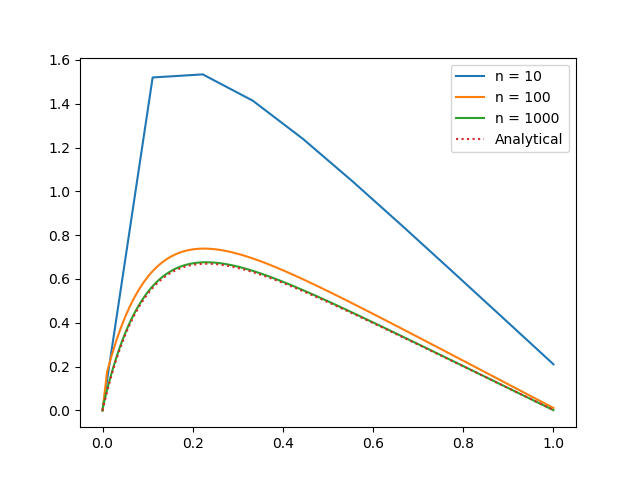
\includegraphics[width=\textwidth]{plot1b.png}
    \caption{:Numerical plot for different values of n compared to an analytical plot for the soulution of the Poisson equation.}
    \label{fig:plot1b}
\end{center}
\end{figure}


\subsection*{Project 1 c)}

Our matrix now have identical elements along the diagonal and identical values for the non diagonal elements, it will look like the matrix below, with $a=-1$ and $b=2$:

\begin{flalign*}
  \begin{bmatrix}
    b & a & 0 &\dots & 0 & 0\\
    a & b & a & \dots & 0 & 0\\
    0 & a & b &  \dots & 0 & 0 \\
    \vdots & \vdots & \vdots & \ddots & \vdots & \vdots \\
    0 & 0 & 0 &\dots& b & a\\
    0 & 0 & 0 &\dots& a & b
  \end{bmatrix}
\end{flalign*}

We develope the algortihm for the forward substitution in the same way as earlier, so the algorithm will be as followed. Here $\tilde{b}_1 = b = 2$ and the algorithm will run with $i$ starting from 2 and going up to $n$.

\begin{flalign*}
  \begin{aligned}
    \tilde{b_i} &= b - \frac{a^2 + (i-2)}{b + (i-2)} \\
    &= 2 - \frac{i-1}{i}
  \end{aligned},
  \qquad \qquad
  \begin{aligned}
    \tilde{g_i} &= g_i - \frac{a}{\tilde{b}_{i-1}}g_{i-1}\\
    &= g_i + \frac{g_{i-1}}{\tilde{b}_{i-1}} \\
  \end{aligned}
\end{flalign*}

where $\tilde{b}_1 = b$ and $\tilde{g}_1 = g$.

\vspace{0.2cm}

Likewise the algorithm for the bacward substitution will be:

\begin{flalign*}
  \begin{aligned}
    u_i &= \tilde{g}_i - \frac{a}{\tilde{b}_i} v_{i+1}\\
    &= \tilde{g}_i + \frac{v_{i+1}}{\tilde{b}_i}
  \end{aligned},
\end{flalign*}

The number of floating points for this special case are $O(7n)$. So we can assume this algorithm will be faster than the general tridiagonal matrix in task b). The CPU time for the two algorithms also shows this as the general matrix took 0.028154 seconds while the special case took 0.024463 seconds for $n = 10^6$.


\subsection*{Project 1 d)}
To compute the relative error in the data set $i = 1,...,n$ we set up:
\[
\epsilon_i = log_{10}(|\frac{v_i - u_i}{u_i}|)
\]

The max values for the relative errors for the matrix in task b) are represented in table 1 below. For $n=10^7$ the error is approching zero, thus the error is decreasing when $n$ is increasing.

\begin{table}[h!]
  \begin{center}
    \caption{ :Relative errors for the general tridiagonal matrix.}
    \label{tab: table1}
    \begin{tabular}{l|r}
      \textbf{n} & \textbf{Max error}\\
      10 & 0.301744 \\
      100 & 0.0374884  \\
      1000 & 0.00384884 \\
      10^7 &   \approx{0}  \\
    \end{tabular}
  \end{center}
\end{table}}

\subsection*{Project 1 e)}

The LU decomposition uses approximately $\frac{2}{3}n^3$ floating points operations to solve a set of linear equations. The differences in the executing time for the LU decomposition and the Thomas algoritm are showed below in Table 2. If we try to run the LU decomposition for a matrix of the size $10^5$ x $10^5$, we get an error message that tells us that the matrix is to large. We can run matrixes on this size with the forward and backward substitutions so this shows that the LU decomposition is a prossess that requires more from the computer than the Thomas algoritm does.

\begin{table}[h!]
  \begin{center}
    \caption{ :Execution time in seconds for solving linear equations with the LU decomposition and the Thomas algortihm.}
    \label{tab:LU}
    \begin{tabular}{c|c|c}
      \textbf{Size of matrix} & \textbf{LU decomposition(sec)} & \textbf{Thomas algoritm(sec)}\\
      10 x 10 & 0.000114 & 2 x 10^{-6} \\
      100 x 100 & 0.001317 & 7 x 10^{-6}\\
      1000 x 1000 & 0.440127 & 2.4 x 10^{-5} \\
    \end{tabular}
  \end{center}
\end{table}}



\subsection*{Comments}
Our group think the first exercise of this project was a bit hard to get started with. Maybe it would be nice to split exercise a) into several parts so it would be easier to get started. When we nailed exercise a) the rest of the project was way smoother.

\subsection*{Appendix}


\href{{https://github.com/emmernme/MENA-Compfys/blob/master/Project%201/QT/main.cpp}}{Link for the main code}


\href{https://github.com/emmernme/MENA-Compfys/blob/master/Project%201/QT/plot.py}{Link to plot-code}


\end{document}
